\section{Simulation Analysis}
\label{sec:simulation}

\subsection{Operating Point Analysis}

\subsection{Step 1 : OP Analysis}

Table~\ref{tab:op1} shows the o

\begin{table}[H]
  \centering
  \begin{tabular}{|l|r|}
    \hline    
    {\bf Name} & {\bf Value [A or V]} \\ \hline
    \input{../sim/op1_tab}
  \end{tabular}
  \caption{Operating point. Variables v(i) are of type {\it voltage} and expressed in
    Volt; other variables are of type {\it current} and expressed in Ampere}
  \label{tab:op1}
\end{table}

The results are the same as the ones obtained using Octave. As the model used is the same. 
It is in stacionary regime, so linear equations used.


\subsection{Step 2: OP Analysis}

Table~\ref{tab:op2}

\begin{table}[H]
  \centering
  \begin{tabular}{|l|r|}
    \hline    
    {\bf Name} & {\bf Value [A or V]} \\ \hline
    \input{../sim/op2_tab}
  \end{tabular}
  \caption{Operating point. Variables v(i) are of type {\it voltage} and expressed in
    Volt; other variables are of type {\it current} and expressed in Ampere}
  \label{tab:op2}
\end{table}

The results are very similar as the ones obtained using Octave. As the model used is the same. 
It is in stacionary regime, so linear equations used.



\subsection{Step 3: Transient Analysis}

Figure~\ref{fig:trans_al3} Transient Analysis

\begin{figure}[H] \centering
  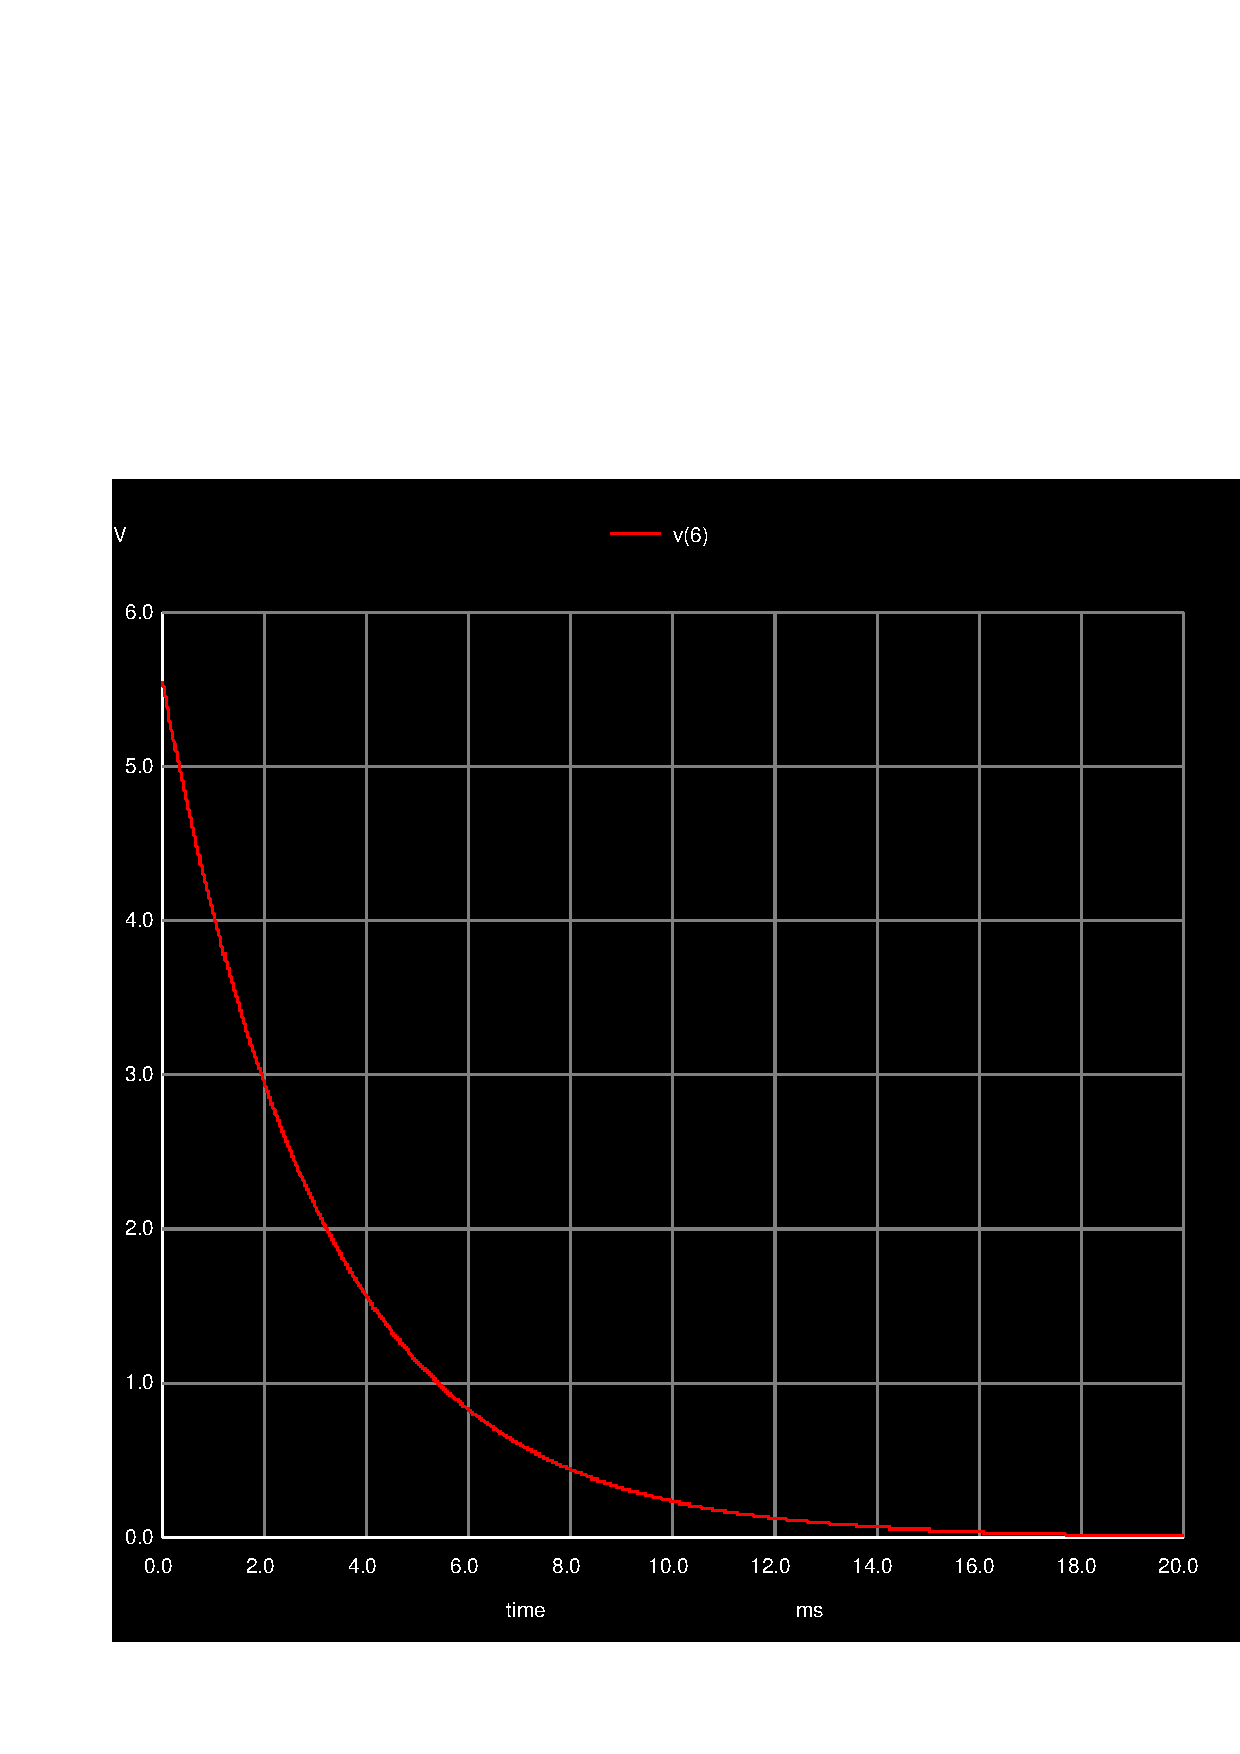
\includegraphics[width=0.6\linewidth]{trans_alinea3.pdf}
  \caption{Transient output voltage of node 6 }
  \label{fig:trans_al3}
  \end{figure}


  Results differ slightly as this involves aproximation of derivatives. The method used is therefore diferent.


\subsection{Step 4: Transient Analysis}


\begin{figure}[H] \centering
  \includegraphics[width=0.6\linewidth]{trans_alinea4.pdf}
  \caption{ Transient analysis with capacitor and Vs as in diagram 1}
  \label{fig:trans_al3}
  \end{figure}

Results differ slightly as this involves aproximation of derivatives. The method used is therefore diferent.

\subsection{Step 5: Frequency analysis}


\begin{figure}[H] \centering
  \includegraphics[width=0.6\linewidth]{trans_alinea5.pdf}
  \caption{ Frequency Analysis in Log Scale}
  \label{fig:trans_al3}
  \end{figure}

  Results differ slightly as this involves aproximation of derivatives. The method used is therefore diferent.

